\chapter{Methode}

% Hier halten Sie fest und begründen, welches Vorgehensmodell Sie für Ihr Projekt wählen. Sie
% verweisen allenfalls auf die daraus entstandenen, konkreten Terminpläne mit Meilensteinen, welche
% z.B. unter Realisierung (Kapitel 5) oder im Anhang versorgt sind.
% Bei Projekten mit einer verlangten wissenschaftlichen Tiefe werden hier die geplanten
% Forschungsmethoden wie quantitative/qualitative Interviews, Befragungen, Beobachtungen,
% Feldexperiment etc. beschrieben und begründet.
% Warum ist in Ihrer Situation ein Interview besser als eine Umfrage? Wer soll interview werden?
% 2(Sie können bei Bedarf in Absprache mit Ihrer Betreuungsperson dazu auch ein zusätzliches
% Methodencoaching beziehen).
% Bei Engineering-Projekten halten Sie weitere einzusetzende fachliche Methoden oder Techniken fest.
% Bei einem Softwareprojekt können dies z.B. der geplante Einsatz einer Anforderungsanalyse, der
% Einsatz von Review-Techniken (Architektur-Reviews) oder bekannter Programmiertechniken sein.
% Dazu gehört auch eine Teststrategie (wo setzen Sie im Projekt Schwerpunkte betr. Testen?). Die
% eigentliche Testdurchführung ist dann unter Realisierung, im Anhang oder einem selbstständigen
% Testdokument beschrieben.

% TODO Nach eigenen Bedürfnissen erweitern
% ------------------------------------- TEIL Wissenschaftliche Arbeiten ----------------------------------------------------
\subsection{Laborexperiment}
% quantitaiv, ehter verhaltenswissenschaftlich als konstruktiv

% Das Experiment untersucht Kausalzusammenhängein kontrollierter Umgebung, indem
% eine Experimen-talvariable auf wiederholbare Weise manipuliert unddie Wirkung
% der Manipulation gemessen wird. DerUntersuchungsgegenstand wird entweder in
% seiner na-türlichen Umgebung (im »Feld«) oder in künstlicherUmgebung (im
% »Labor«) untersucht, wodurch wesentlichdie Möglichkeiten der Umgebungskontrolle
% beeinflusstwerden. (Balzert, S. 286)

% ------------------------------------- TEIL Ingenieurlastige Arbeiten ----------------------------------------------------
\section{Projektinformationen}

In diesem Abschnitt wird aufgezeigt welches Vorgehensmodell und welche Methoden verwendet wurden zur Abwicklung dieses Projektes.
Auch wird aufgezeigt wie das Projekt organisiert ist.

\subsection{Vorgehensmodell}

% TODO: vorgehensmodell festsetzen
% SoDa? KanBan? Quellen?


\subsection{Projektteam}

Die folgende Tabelle~\ref{tab:projectmembers} listet alle Personen auf die an diesem Projekt beteiligt sind.

\begin{table}[H]
    \begin{tabular}{l p{3.2cm}}
        \toprule
        \bfseries Person   & \bfseries Rollen \\
        \midrule
        Konrad Bächler     & Auftraggeber \\
        \midrule
        Carolyn Bächler    & Auftraggeber \\
        \midrule
        Arnold Dieter      & Betreuungsperson \\
        \midrule
        tbd.               & Experte \\
        % TODO: find out who's the expert
        \midrule
        Moritz Küttel      & Student \\
        \bottomrule
    \end{tabular}
    \caption{People involved in the project}\label{tab:projectmembers}
\end{table}

\subsection{Quellcode}

Der \LaTeX-Quellcode für diesen Bericht ist auf codeberg.org in diesem Repository zu finden:
\url{https://codeberg.org/mkuettel/ba}

%TODO: add links to all the source code

\subsection{Projektboard und Issue-Tracker}

Die Abbildung~\ref{fig:projectboard} zeigt das Projektboard, welches für Projektmanagement und Controlling verwendet wird.
Jede Karte auf dem Projektboard ist ein Issue aus dem Issue-Tracker:

\url{https://codeberg.org/mkuettel/ba/issues}

Der Issue-Tracker ist zugleich ein Backlog. Issues können nach Bedarf aus dem BackLog entnommen werden und zum Projektboard hinzugefügt werden.

Das Projektboard ist ein KanBan-Board und enthält drei Spalten: ''To Do'', ''In Progress'' und ''Done''.
Diese Issues aus dem Issue-Tracker können dann je nach fortschritt in die Spalten einsortiert werden. 
Ziel von KanBan ist es eines nach dem anderen zu machen und sich auf einen Task zu fokussieren. Man sollte also nie mehr als einen Issue in der Spalte ''In Progress'' haben.
%TODO: definition of done
% https://de.wikipedia.org/wiki/Kanban_(Softwareentwicklung)

%TODO: describe how issues are categorized (labels, milestones, projects etc.)

Das KanBan-Board ist hier zu finden:

\url{https://codeberg.org/mkuettel/BA/projects/125}


\begin{figure*}[ht]
    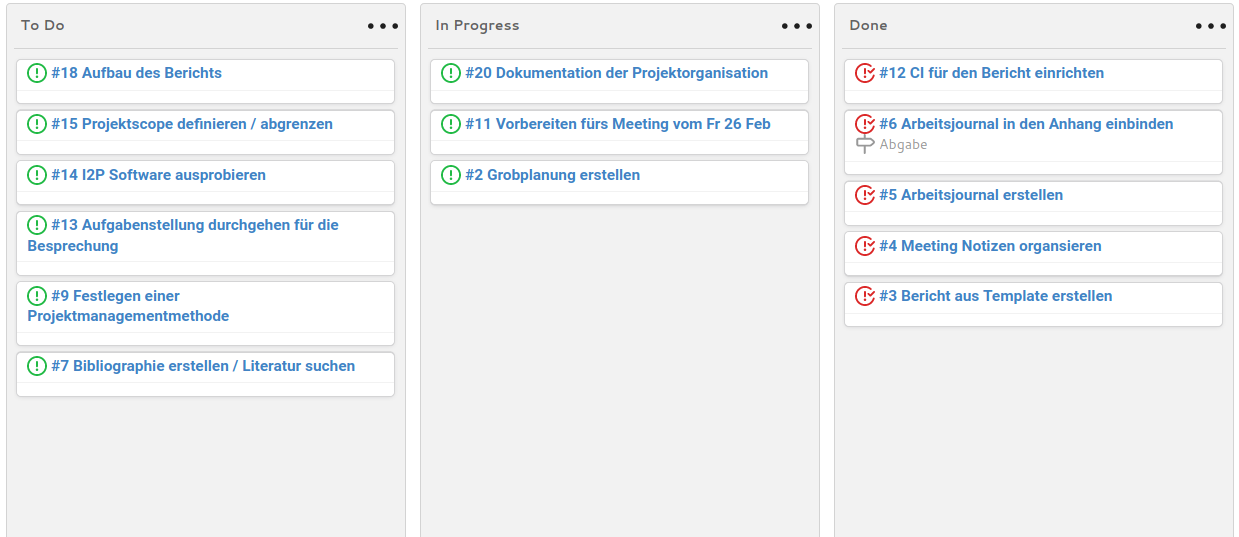
\includegraphics[width=1.0\textwidth]{project-board.png}
    \caption{CodeBerg Project Board}
    \label{fig:projectboard}
\end{figure*}


Ein einziger Issue sollte nie mehr Aufwand machen als acht Stunden Arbeit. Diese Regel hilft die Issues kleiner zu halten und genauere Aussagen treffen zu können, wo man im Projekt steht.

Wird an einem Issue gearbeitet wird dies im Journal vermerkt \& in der Git-Historie hinterlegt.
Das Arbeitsjournal ist im Anhang~\ref{sec:journal} zu finden.


Die Länge eines Sprints in KanBan ist nicht genau definiert, sondern der Sprint ist fertig wenn alle Arbeit für den jeweiligen Sprint erledigt wurde.

\subsection{Ermittlung offener Projektrahmenbedingungen}
\label{ch:evaluation}

% TODO: Requirements engineering Methode

\subsection{Projektanforderungen / Anforderungsanalyse}
\label{sub:Anforderungen}

\subsection{Einschränkungen und Abgrenzungen}

% TODO: Scope in der Einleitung
% TODO: Scope definieren

\subsection{Systemarchitektur}

\subsection{Komponentendesign}

\subsection{Umsetzung / Programmierung}

\subsection{Testing}
